\documentclass{ximera}

\graphicspath{  
{./}
{./whoAreYou/}
{./drawingWithTheTurtle/}
{./bisectionMethod/}
{./circles/}
{./anglesAndRightTriangles/}
{./lawOfSines/}
{./lawOfCosines/}
{./plotter/}
{./staircases/}
{./pitch/}
{./qualityControl/}
{./symmetry/}
{./nGonBlock/}
}


%% page layout
\usepackage[cm,headings]{fullpage}
\raggedright
\setlength\headheight{13.6pt}


%% fonts
\usepackage{euler}

\usepackage{FiraMono}
\renewcommand\familydefault{\ttdefault} 
\usepackage[defaultmathsizes]{mathastext}
\usepackage[htt]{hyphenat}

\usepackage[T1]{fontenc}
\usepackage[scaled=1]{FiraSans}

%\usepackage{wedn}
\usepackage{pbsi} %% Answer font


\usepackage{cancel} %% strike through in pitch/pitch.tex


%% \usepackage{ulem} %% 
%% \renewcommand{\ULthickness}{2pt}% changes underline thickness

\tikzset{>=stealth}

\usepackage{adjustbox}

\setcounter{titlenumber}{-1}

%% journal style
\makeatletter
\newcommand\journalstyle{%
  \def\activitystyle{activity-chapter}
  \def\maketitle{%
    \addtocounter{titlenumber}{1}%
                {\flushleft\small\sffamily\bfseries\@pretitle\par\vspace{-1.5em}}%
                {\flushleft\LARGE\sffamily\bfseries\thetitlenumber\hspace{1em}\@title \par }%
                {\vskip .6em\noindent\textit\theabstract\setcounter{question}{0}\setcounter{sectiontitlenumber}{0}}%
                    \par\vspace{2em}
                    \phantomsection\addcontentsline{toc}{section}{\thetitlenumber\hspace{1em}\textbf{\@title}}%
                     }}
\makeatother



%% thm like environments
\let\question\relax
\let\endquestion\relax

\newtheoremstyle{QuestionStyle}{\topsep}{\topsep}%%% space between body and thm
		{}                      %%% Thm body font
		{}                              %%% Indent amount (empty = no indent)
		{\bfseries}            %%% Thm head font
		{)}                              %%% Punctuation after thm head
		{ }                           %%% Space after thm head
		{\thmnumber{#2}\thmnote{ \bfseries(#3)}}%%% Thm head spec
\theoremstyle{QuestionStyle}
\newtheorem{question}{}



\let\freeResponse\relax
\let\endfreeResponse\relax

%% \newtheoremstyle{ResponseStyle}{\topsep}{\topsep}%%% space between body and thm
%% 		{\wedn\bfseries}                      %%% Thm body font
%% 		{}                              %%% Indent amount (empty = no indent)
%% 		{\wedn\bfseries}            %%% Thm head font
%% 		{}                              %%% Punctuation after thm head
%% 		{3ex}                           %%% Space after thm head
%% 		{\underline{\underline{\thmname{#1}}}}%%% Thm head spec
%% \theoremstyle{ResponseStyle}

\usepackage[tikz]{mdframed}
\mdfdefinestyle{ResponseStyle}{leftmargin=1cm,linecolor=black,roundcorner=5pt,
, font=\bsifamily,}%font=\wedn\bfseries\upshape,}


\ifhandout
\NewEnviron{freeResponse}{}
\else
%\newtheorem{freeResponse}{Response:}
\newenvironment{freeResponse}{\begin{mdframed}[style=ResponseStyle]}{\end{mdframed}}
\fi



%% attempting to automate outcomes.

%% \newwrite\outcomefile
%%   \immediate\openout\outcomefile=\jobname.oc
%% \renewcommand{\outcome}[1]{\edef\theoutcomes{\theoutcomes #1~}%
%% \immediate\write\outcomefile{\unexpanded{\outcome}{#1}}}

%% \newcommand{\outcomelist}{\begin{itemize}\theoutcomes\end{itemize}}

%% \NewEnviron{listOutcomes}{\small\sffamily
%% After answering the following questions, students should be able to:
%% \begin{itemize}
%% \BODY
%% \end{itemize}
%% }
\usepackage[tikz]{mdframed}
\mdfdefinestyle{OutcomeStyle}{leftmargin=2cm,rightmargin=2cm,linecolor=black,roundcorner=5pt,
, font=\small\sffamily,}%font=\wedn\bfseries\upshape,}
\newenvironment{listOutcomes}{\begin{mdframed}[style=OutcomeStyle]After answering the following questions, students should be able to:\begin{itemize}}{\end{itemize}\end{mdframed}}



%% my commands

\newcommand{\snap}{{\bfseries\itshape\textsf{Snap!}}}
\newcommand{\flavor}{\link[\snap]{https://snap.berkeley.edu/}}
\newcommand{\mooculus}{\textsf{\textbf{MOOC}\textnormal{\textsf{ULUS}}}}


\usepackage{tkz-euclide}
\tikzstyle geometryDiagrams=[rounded corners=.5pt,ultra thick,color=black]
\colorlet{penColor}{black} % Color of a curve in a plot



\ifhandout\newcommand{\mynewpage}{\newpage}\else\newcommand{\mynewpage}{}\fi


\author{Jenny Sheldon \and Bart Snapp}


\outcome{Explain what is meant by a reflection.}
\outcome{Compute reflections using matrix multiplication.}
\outcome{Use the distance formula to show that a given reflection is an isometry.}

\title{Reflections}

\begin{document}
\begin{abstract}
  We view reflections as matrices.
\end{abstract}
\maketitle

The act of reflection has fascinated humanity for millennia.  It has a
strong effect on our perception of beauty and has a defined place in
art---not to mention how useful it is for the application
of make-up. Here is our definition of a reflection:

\begin{definition}
The \dfn{reflection} across a line $\l$, denoted by $\mat{F}_\l$, is the
function that maps a point $\vec{p}$ to a point $\mat{F}_\l
\vec{p}$ such that:
\begin{enumerate}
\item If $\vec{p}$ is on $\l$, then $\mat{F}_\l \vec{p} = \vec{p}$.
\item If $\vec{p}$ is not on $\l$, then $\l$ is the perpendicular
  bisector of the segment connecting $\vec{p}$ and $\mat{F}_\l \vec{p}$. 
\end{enumerate}
\end{definition}

You might be saying, ``Huh?''  It's not as hard as it looks.  Check
out this picture of the situation; again Louie Llama\index{Louie Llama} 
will help us out:
\begin{image}
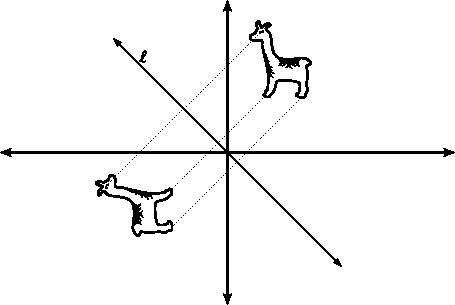
\includegraphics{refIdeaEg.pdf}
\end{image}

\subsubsection{A Collection of Reflections}

We are going to begin with a trio of reflections. We'll start with a
\textbf{horizontal reflection}\index{horizontal reflection}\index{reflection!horizontal} across the $y$-axis.  Using
our matrix notation, we write:
\[
\mat{F}_{x=0} =
\begin{bmatrix}
-1 & 0 & 0\\
 0 & 1 & 0\\
 0 & 0 & 1
\end{bmatrix}
\]

The next reflection in our collection is a \textbf{vertical
  reflection}\index{vertical reflection}\index{reflection!vertical}
across the $x$-axis.  Using our matrix notation, we write:
\[
\mat{F}_{y=0} =
\begin{bmatrix}
1 &  0 & 0\\
0 & -1 & 0\\
0 &  0 & 1
\end{bmatrix}
\]
The final reflection to add to our collection is a \textbf{diagonal
  reflection}\index{diagonal reflection}\index{reflection!diagonal}
across the line $y=x$.  Using our matrix notation, we write:
\[
\mat{F}_{y=x} =
\begin{bmatrix}
0 & 1 & 0\\
1 & 0 & 0\\
0 & 0 & 1
\end{bmatrix}
\]


\begin{example}
Consider the point $\vec{p} =(3,-1)$.  Use a matrix to reflect
$\vec{p}$ across the line $y = x$.
\begin{image}
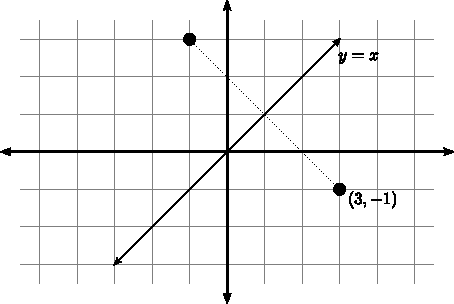
\includegraphics{refEg1.pdf}
\end{image}
Here is how you do it:
\begin{align*}
\mat{F}_{y = x} \vec{p} &= 
\begin{bmatrix}
0 & 1 & 0 \\ 
1 & 0 & 0 \\
0 & 0 & 1
\end{bmatrix}
\begin{bmatrix}
3 \\
-1 \\
1
\end{bmatrix}\\
&=
\begin{bmatrix}
0-1+0\\
3+0+0 \\
0+0+1
\end{bmatrix}\\
&=
\begin{bmatrix}
-1\\
3 \\
1
\end{bmatrix}
\end{align*}
Hence we end up with the point $(-1,3)$. 
\end{example}

\begin{question}
Let $\vec{p}$ be some point in Quadrant I of the $(x,y)$-plane. What
reflection will map this point to Quadrant II? What about Quadrant IV?
What about Quadrant III?
\end{question}



\begin{question} 
Can you demonstrate with algebra why each of our reflections above are
isometries?
\end{question}



\end{document}
